\documentclass[../poliXuniversity_hospital_(USP)_report.tex]{subfiles}

\begin{document}
\chapter{Hardware Ciclo}

\section{Estrutura Mecânica}

\subsection{Estrutura mecânica e fixação}

Para oferecer estabilide e suporte mecânico durante o exercício foi desenvolvido um mecanismo de compressão do leito de UTI, no qual usando morças e manípulos é possivel ajustar a compressaõ e garantir estabilidade e flexibilidade na hora de acoplar a diferentes leitos. Foram usados perfis de alumínio 20x20 v-slot, chapas de MDF para base e impressões 3D em PLA para demais componentes, além disso foi usado o pedal e suporte de uma bicicleta ergonômica genérica(WCT)

\begin{figure}[h]
\centering
    \begin{minipage}{0.5\textwidth}
        \centering
        \caption{Bicicleta cicloergométrica WCT fitness}
        \centering % para centralizarmos a figura
        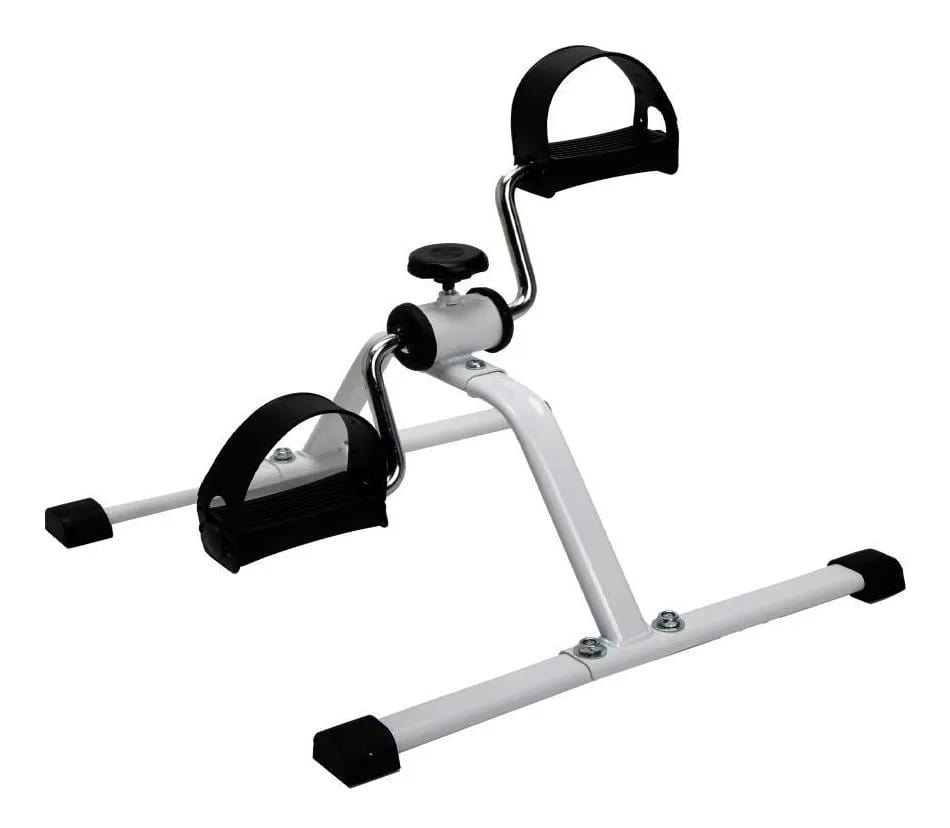
\includegraphics[width=5cm]{images/WCT_ciclo.jpg}
        \caption*{Fonte: Mercado Livre}
        \label{figura: icicleta cicloergométrica WCT fitness}
        
    \end{minipage}\hfill
    \begin{minipage}{0.5\textwidth}
    
        \centering
        \caption{Ciclo Ergômetro no Leito (CAD)}
        \centering % para centralizarmos a figura
        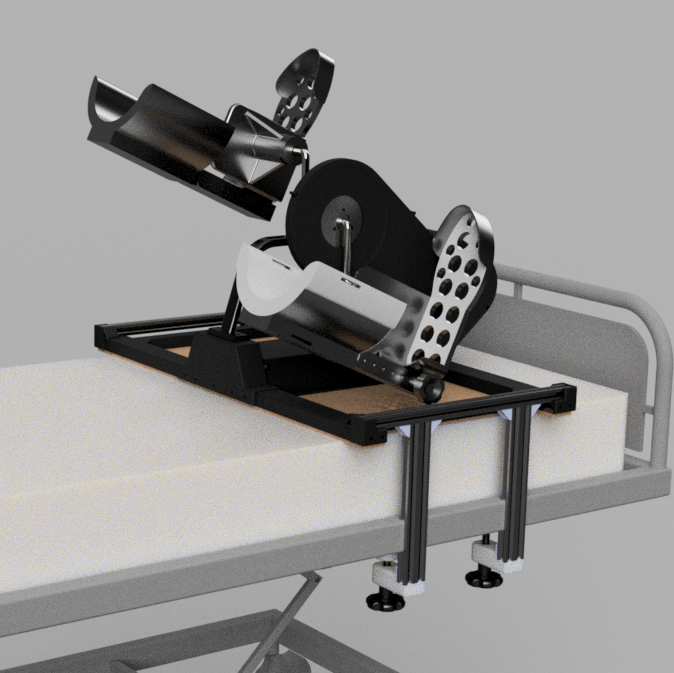
\includegraphics[width=5cm]{images/ciclo_leito.png}
        \caption*{Fonte: Autor}
        \label{figura: Ciclo Ergômetro no Leito (CAD)}
        
    \end{minipage}\hfill
\end{figure}

\subsection{Mecanismo de rotação e pedalada}
No mecanismo de pedala, foi desenvolvido e fabricado uma polia bipartida e foi soldada ao eixo do pedal, tal polia possui os furos para acoplar uma coroa e assim transmitir o torque vindo do motor

\begin{figure}[h]
\centering
    \begin{minipage}{0.5\textwidth}
        \centering
        \caption{Polia bipartida}
        \centering % para centralizarmos a figura
        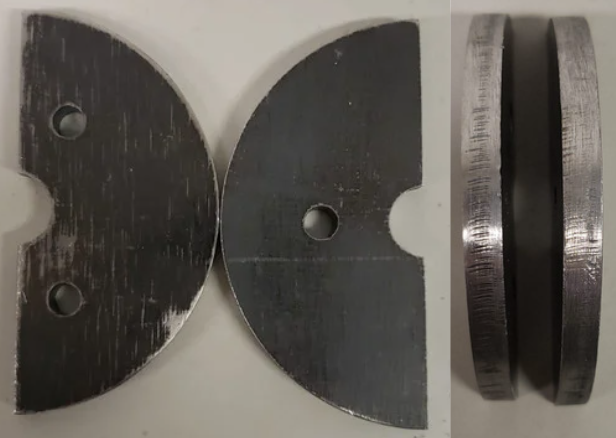
\includegraphics[width=7cm]{images/poliabipartida.png}
        \caption*{Fonte: Autor}
        \label{figura: Polia bipartida}
        
    \end{minipage}\hfill
    \begin{minipage}{0.5\textwidth}
    
        \centering
        \caption{Transmissão por corrente ciclo}
        \centering % para centralizarmos a figura
        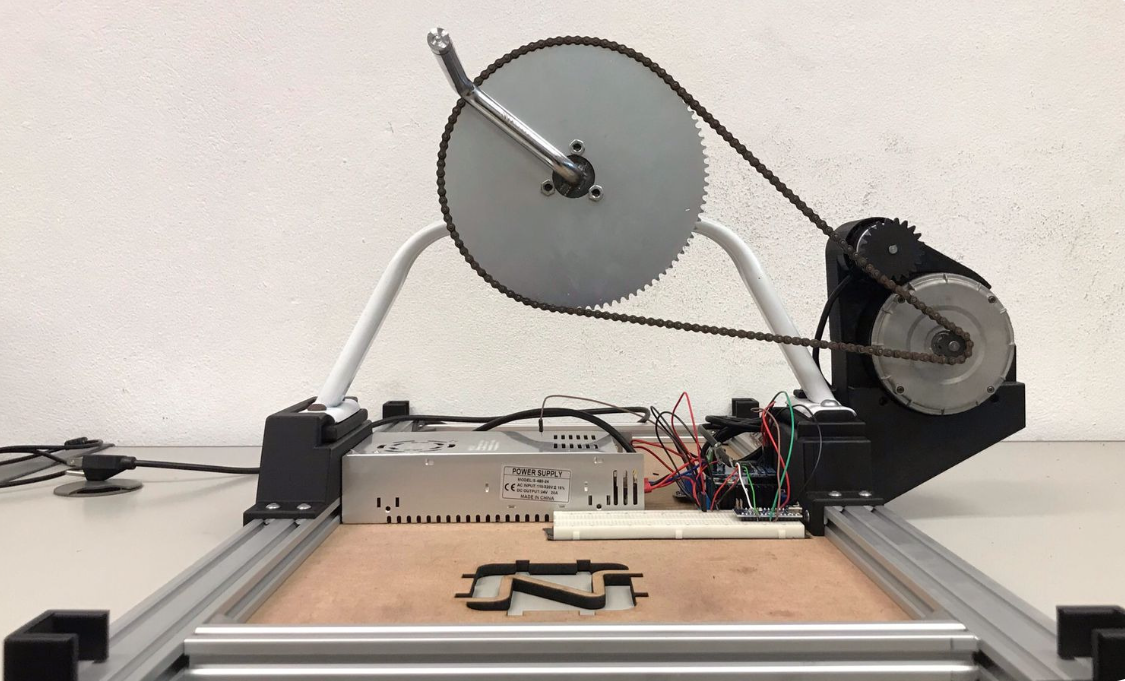
\includegraphics[width=7cm]{images/tração_ciclo.png}
        \caption*{Fonte: Autor}
        \label{figura: Transmissão por corrente ciclo}
        
    \end{minipage}\hfill
\end{figure}

\subsection{Pedais ergonômico}

importante fator para pacientes de mobilidade reduzida é um aparelho ergonômico que garanta bom posicionamento do joelho e panturilha. Para evitar lesões durante o movimento e o máximo conforto possível foi desenvolvido um pedal que se assemelha a uma bota, na qual é possivel segurar panturilha e pé.

\begin{figure}[h]
\centering
\caption{Pedal Ergonômico}
    \begin{minipage}{0.5\textwidth}
        \centering
        
        \centering % para centralizarmos a figura
        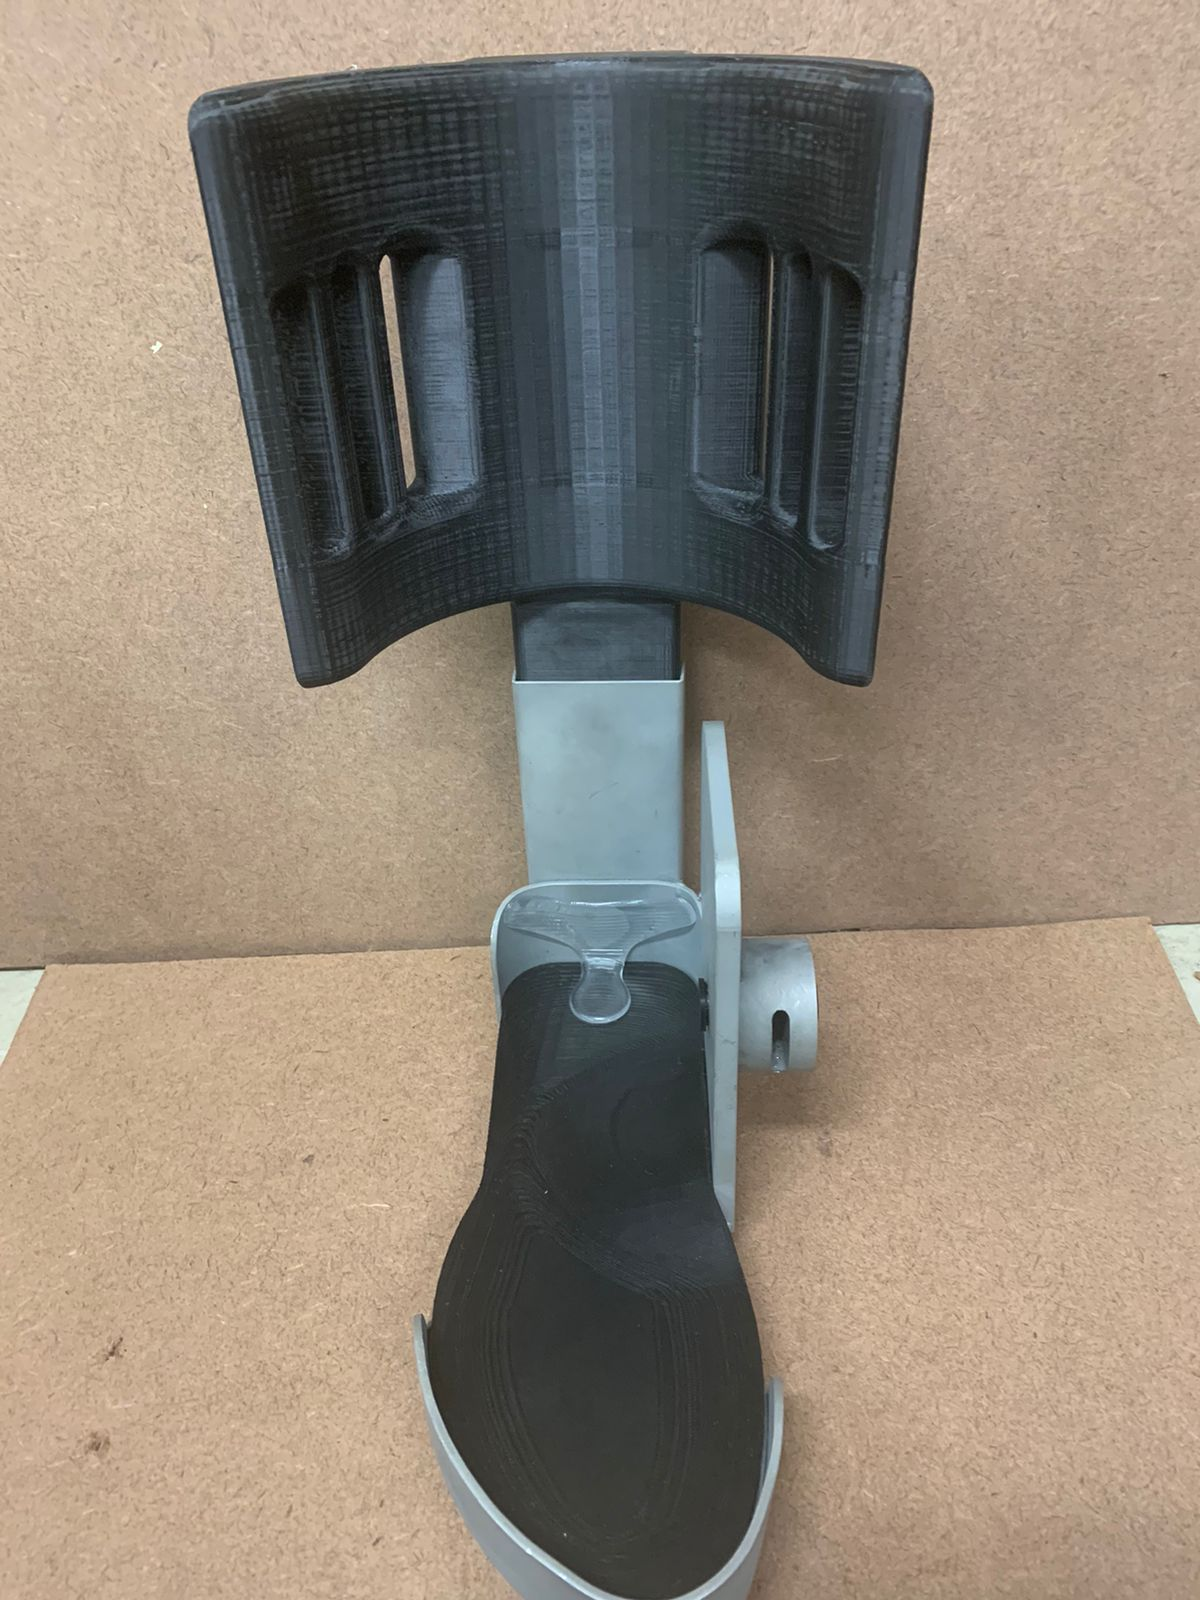
\includegraphics[width=6cm]{images/pedal_angulada.jpeg}
        \label{figura: Pedal angulada}
        
    \end{minipage}\hfill
    \begin{minipage}{0.5\textwidth}
    
        \centering
        \centering % para centralizarmos a figura
        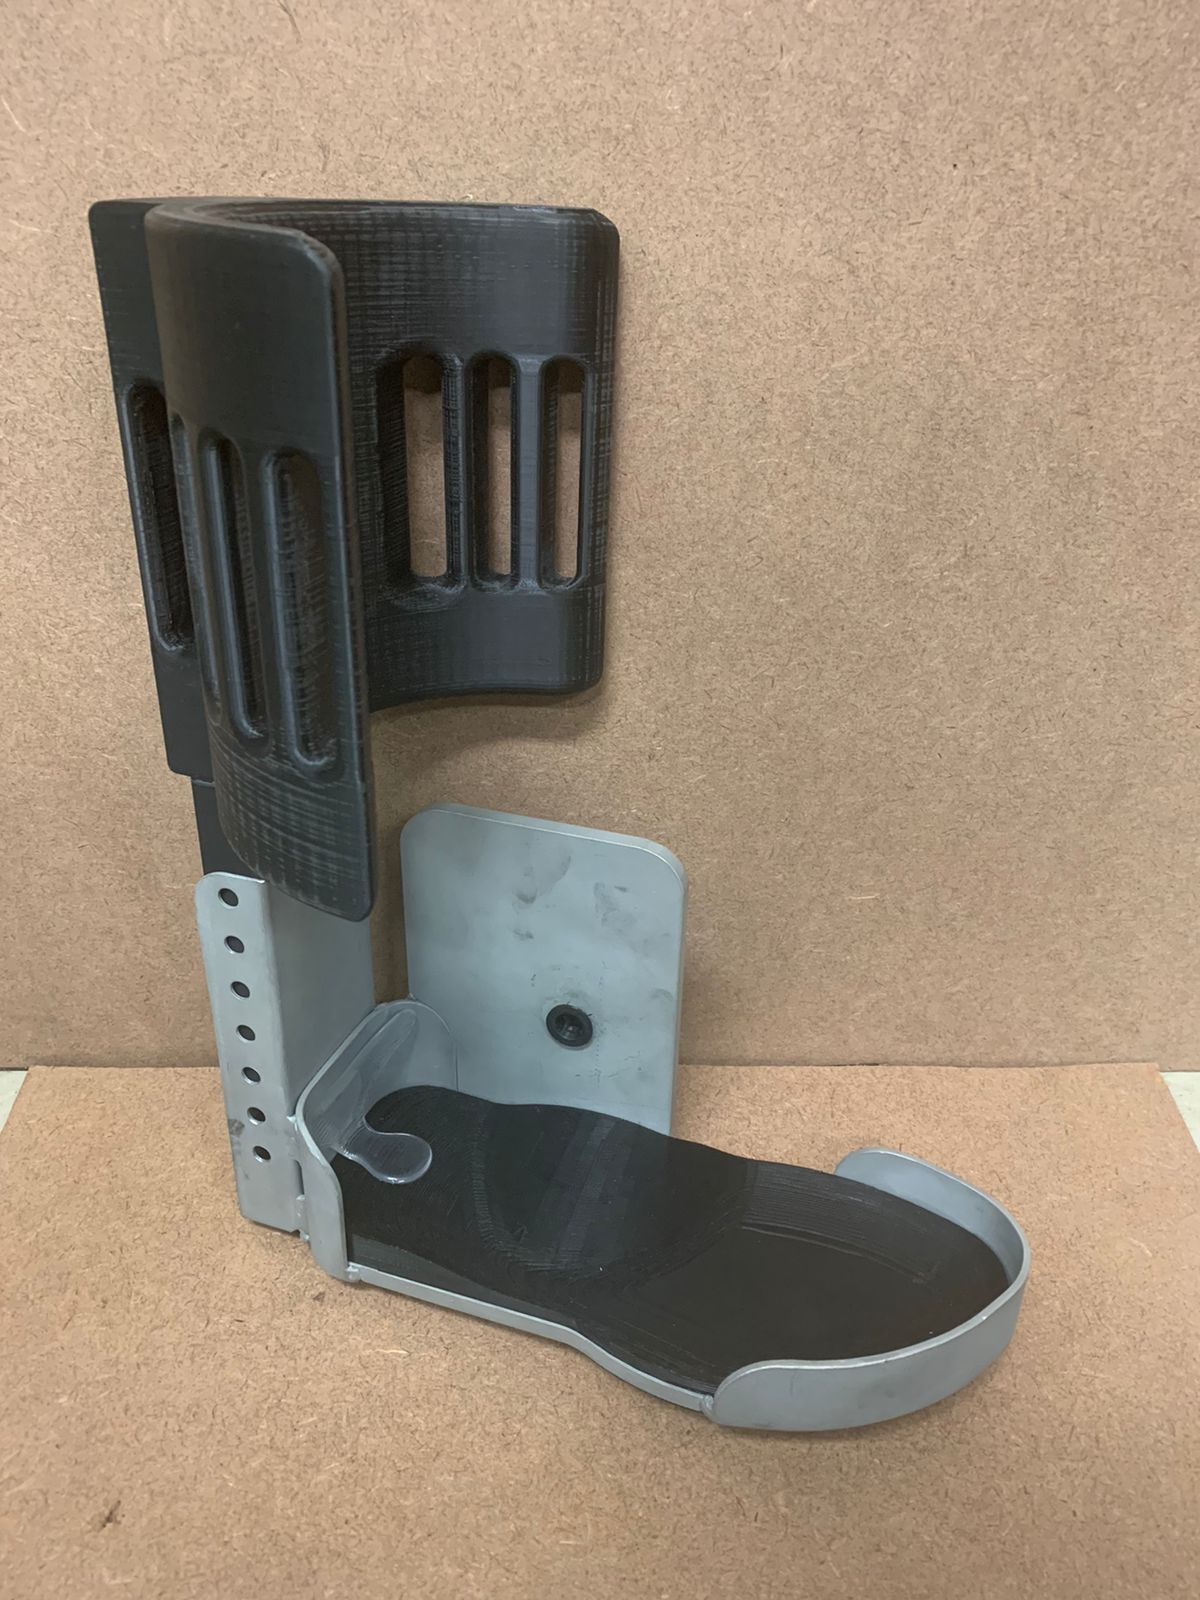
\includegraphics[width=6cm]{images/Pedal_frontal.jpeg}
        
        \label{figura: Pedal frontal}
        
    \end{minipage}\hfill
    \caption*{Fonte: Autor}
\end{figure}

\section{Sistemas Eletrônicos}

\subsection{Distribuição de enregia}
o diagrama abaixo mostra toda distribuição do projeto na qual se basea em um fonte chaveada 24V 30A, um conversor de tensão o qual transforma 24V em 5V e assim alimenta todos os elementos exceto pelo motor.Tanto a fonte quanto o conversor ja foram citados.


\begin{figure}[h]
\centering
    \caption{Distribuição de Energia Ciclo}
    \centering % para centralizarmos a figura
    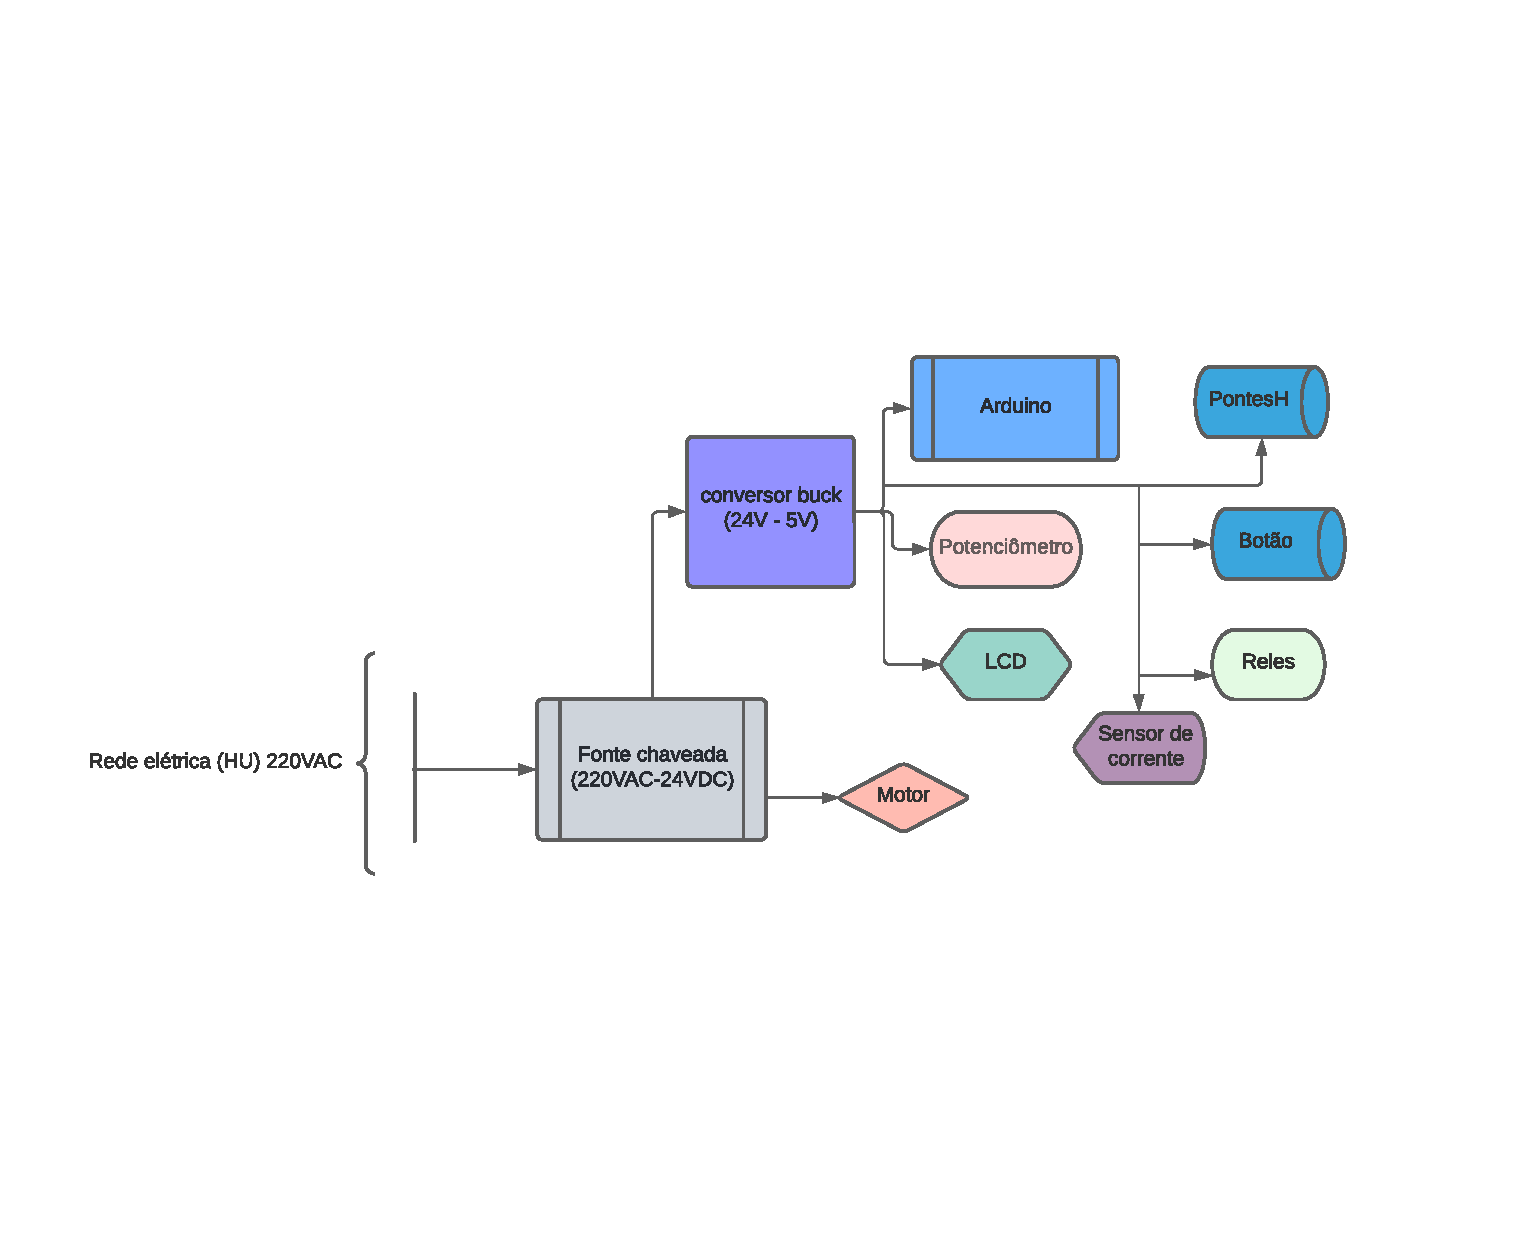
\includegraphics[width=20cm]{images/distribuiçãoenergia.pdf}
    \caption*{Fonte: Distribuição de Energia Ciclo}
    \label{figura: Distribuição de Energia Ciclo}
\end{figure}


\subsection{Sistema de tração}
Foi escolhido o motor DC escovado MB300W devido ao seu torque suficiente mente alto e custo relativamente baixo. Para aumentar o torque do motor e diminuir o RPM foi utilizado uma redução 9:1 com a coroa dentada tipo 95H. Para o controle do motor foi usado a ponte H BTS7960 já citada anteriormente.

\begin{figure}[h]
\centering
    \caption{Motor MB300W24}
    \centering % para centralizarmos a figura
    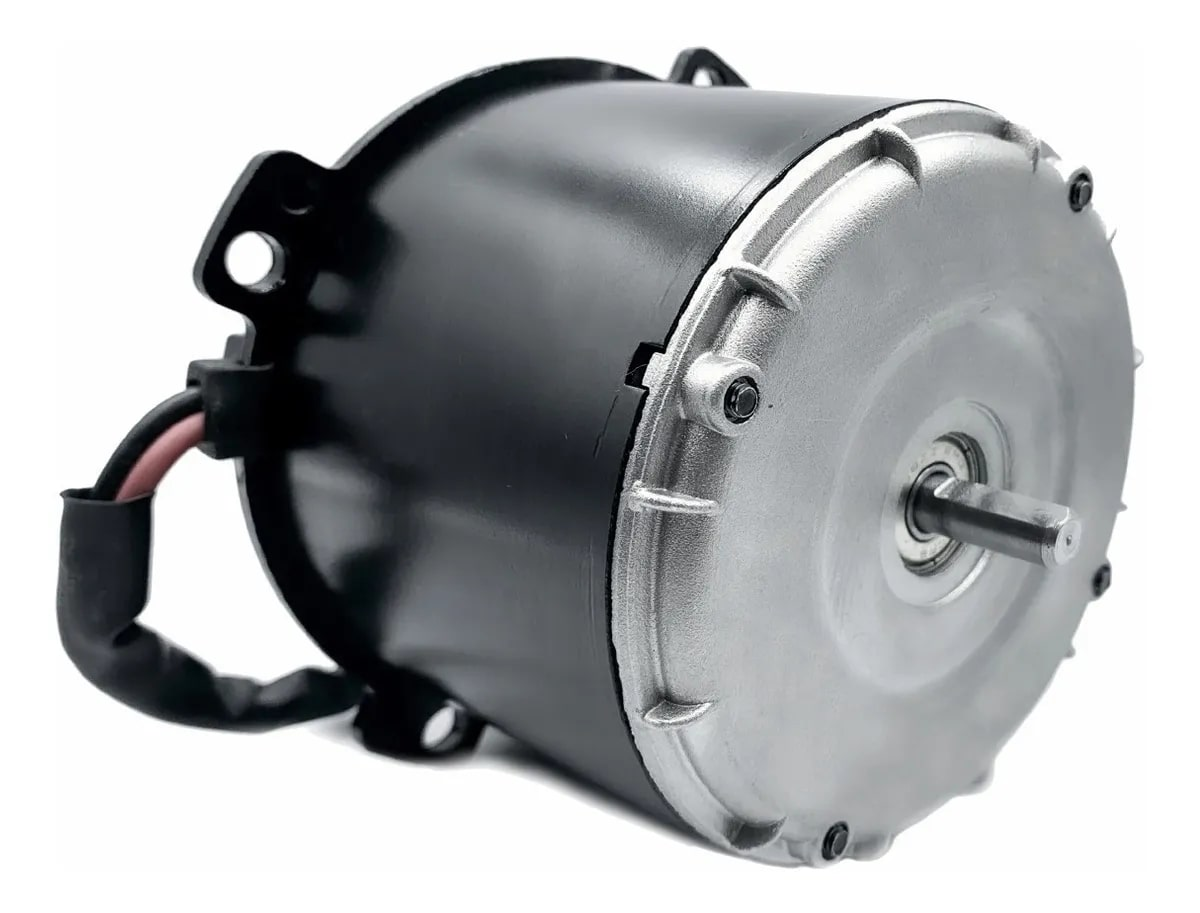
\includegraphics[width=8cm]{images/MB200W24.jpg}
    \caption*{Fonte: Mercado Livre}
    \label{figura: MB300W24}
\end{figure}

\subsection{Módulos embarcados}
Para organizar o projeto eletrônico foi desenvolvido uma placa de circuito impresso que acomodasse o microcontrolador arduino, reles e sensor de corrente e recebesse o sinais do encoder, botão e potenciômetro e comandasse a ponte H e LCD.

\begin{figure}[h]
\centering
    \begin{minipage}{0.5\textwidth}
        \centering
        
        \caption{Módulo Ciclo Ergômetro}
        \centering % para centralizarmos a figura
        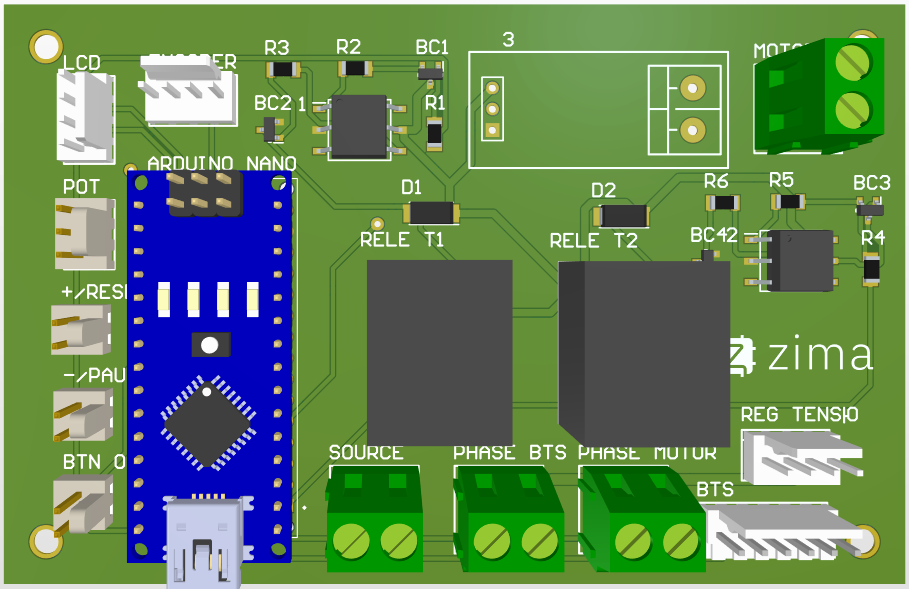
\includegraphics[width=7cm]{images/pcb_ciclo.png}
        \label{figura: Módulo Ciclo Ergômetro}
        
    \end{minipage}\hfill
    \begin{minipage}{0.5\textwidth}
    
        \centering
        \caption{Esquemático Módulo Ciclo}
        \centering % para centralizarmos a figura
        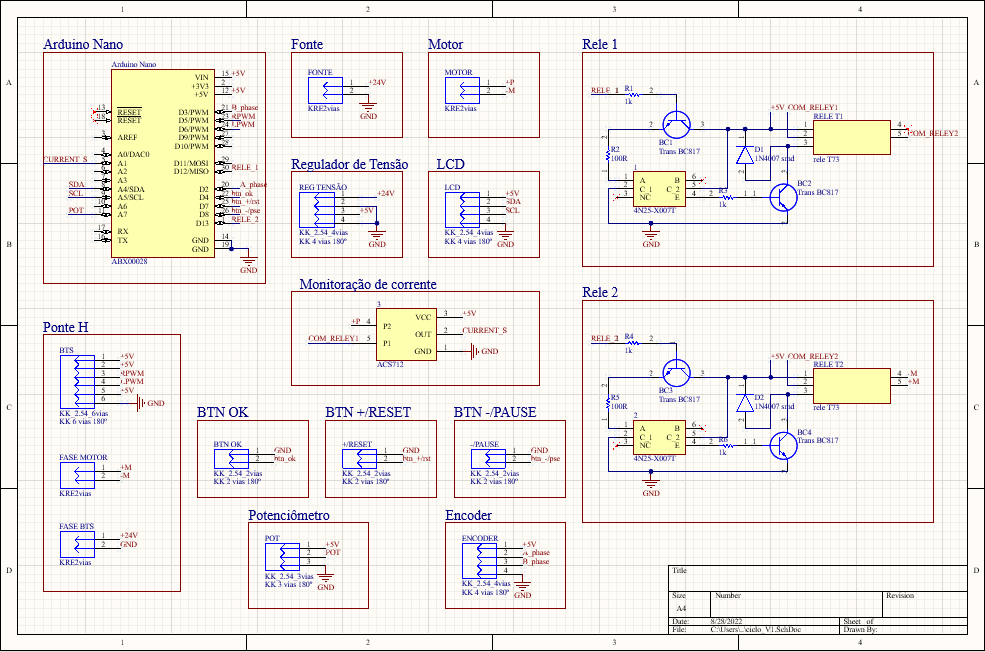
\includegraphics[width=6cm]{images/esquematico_ciclo.png}
        \label{figura: Esquemático Módulo Ciclo}
        
    \end{minipage}\hfill
    \caption*{Fonte: Autor}
\end{figure}

\subsection{Sistema de realimentação}

Para mensurar e controlar parâmetros importantes do processo de reabilitação foi inserido um encoder rotativo, mesmo usado no golgi bot, para leitura do RPM e um sensor de corrente ACS712 20A para estimar o torque através do Kt do motor.

\begin{figure}[h]
\centering
    \caption{ACS712 20A}
    \centering % para centralizarmos a figura
    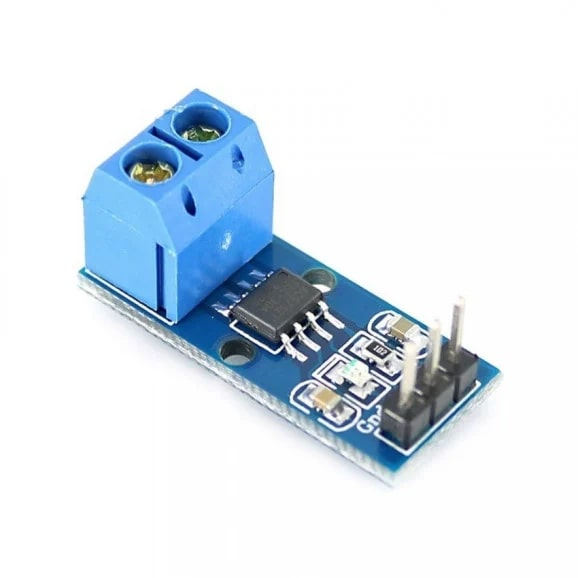
\includegraphics[width=8cm]{images/acs712.jpg}
    \caption*{Fonte: Baú da Eletrônica}
    \label{figura: ACS712 20A4}
\end{figure}

\end{document}